\chapter*{Prologue: Computation Is Transformation}
\addcontentsline{toc}{chapter}{Prologue: Computation Is Transformation}

\label{chap:computation-is-transformation}

I didn't start thinking in graphs because I read a seminal paper, or because I spent my nights studying category theory, or because I had some grand, lightning-strike revelation about the fundamental nature of computation.

I started thinking in graphs because a game studio I worked at had a build system that \textbf{sucked}.

I don't mean "mildly inconvenient" sucked. I mean, we had sixty developers and only three build machines, and every morning the entire studio tried to merge their work into the same shared engine codebase like a stampede of buffalo diving into a single narrow canyon. The congestion was physical; you could feel the heat rising in the room as the queue grew.

If you managed to fix a bug at 11 a.m., good luck seeing it in QA's hands before dinner. The latency loop was measured in hours, not seconds.

And the stakes were high. If you broke the build, you were \textit{that person}—the one who froze the pipeline, stalled the artists, ticked off the designers, and effectively derailed the entire schedule for the day. The "build debacle," as we affectionately called it, wasn't just an annoyance. It was structurally broken.

There were too many people trying to integrate at once, and far too few machines to handle the load. There was no isolation between game teams; a breakage in the physics engine for the racing game would halt the RPG team's ability to test their dialogue system. Visibility was non-existent. Rebuild times were excruciatingly long because the system had no concept of incremental reasoning.

Worst of all, there was no way to ask the most basic questions:
\begin{itemize}
    \item What actually depends on what?
    \item What \textit{needs} to rebuild versus what is already fresh?
    \item Why is this compilation step even happening?
\end{itemize}

So I started digging. Not because I wanted to—because I had to. Someone needed to unfuck the pipeline, and apparently, that someone was me.

I didn't have a plan. I didn't have deep experience writing build systems. I wasn't even "the build guy"—I was just the engineer who couldn't stop asking annoying questions. And the first question I asked—the one that changed everything—was embarrassingly simple:

\textbf{"What \textit{is} a build, really?"}

It's not the shell scripts. It's not the bespoke tools. It's not Jenkins, or the cloud, or the physical racks of servers humming in the closet. 

What \textit{is} it?

\section{The Day I Realized Everything Was a Graph}
\label{sec:day-i-realized}

If you strip away the noise, the implementation details, and the specific syntax of makefiles, a build is essentially three things:
\begin{enumerate}
    \item A collection of inputs (source files, assets, configurations).
    \item A collection of outputs (executables, archives, binaries).
    \item \textbf{A set of transformations that turn one into the other.}
\end{enumerate}

That's it. It is a transformation engine.

You can visualize every build process as a directed flow:
\[
[\text{Assets}] \rightarrow [\text{Compiler}] \rightarrow [\text{Objects}] \rightarrow [\text{Linker}] \rightarrow [\text{Executable}]
\]

Once I started seeing this, I couldn't stop seeing it. You can draw every dependency tree as a graph of ``this depends on that.'' You can draw every version-control history as a DAG of ``this commit comes after that.'' You can even visualize a merge conflict as a topological mismatch between two graph branches.

\begin{figure}[h]
    \centering
    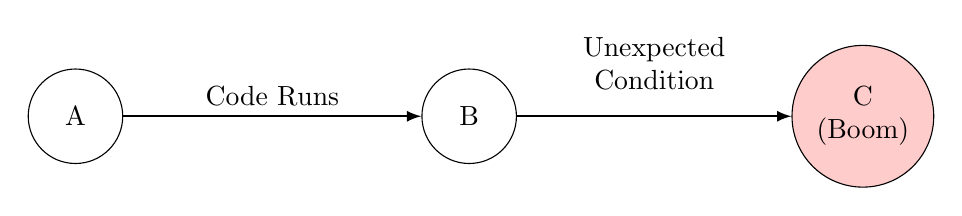
\begin{tikzpicture}[>=latex, node distance=5.0cm]
    \tikzset{
        state/.style={circle, draw, minimum size=1.2cm, align=center},
        boom/.style={circle, draw, minimum size=1.8cm, fill=red!20, align=center}
    }

        \node[state] (A) {A};
        \node[state] (B) [right of=A] {B};
        \node[boom]  (C) [right of=B] {C\\(Boom)};

        \draw[->, thick] (A) -- node[midway, above] {Code Runs} (B);
        \draw[->, thick] (B) -- node[midway, above, yshift=6pt, align=center] {Unexpected\\Condition} (C);

    \end{tikzpicture}

    \caption{A crash bug visualized as a path through state space.}
\end{figure}

Everything I looked at—builds, merges, crashes, asset pipelines, scripts, even the coordination of the humans involved—suddenly made more sense when drawn as nodes and edges. It wasn't a thunderclap epiphany. It was a slow, creeping realization:

\textbf{Everything we build is structure transforming into other structure. And the best way to see structure is to draw it.}

The more problems I solved using this mental model, the more natural it felt. Build steps became nodes. Dependencies became edges. Failures became dead ends. Parallelization became independent branches. Caching was revisiting previously reached nodes.

Git branching? Graph.  
Gameplay systems? Graphs of state transitions.  
NPC behavior trees? Graphs.  
Physics collision islands? Graphs.  
Data flow? Graphs.  
Event pipelines? Graphs.  

Everywhere I looked, the same pattern repeated. And the punchline was this: I didn't choose graphs. The problems chose graphs.

\section{Graphs Reveal What the Code Is Actually Doing}
\label{sec:graphs-reveal}

\begin{center}
{\LARGE\bfseries Computation is a transformation of state.}\\[6pt]
{\Large\bfseries And transformations have geometry.}\\[6pt]
{\large\bfseries Geometry is how computation makes sense.}
\end{center}

We like to pretend code is a set of instructions, a recipe, or a linear list of steps to be followed. But that is a lie we tell ourselves to make the complexity manageable. We write in lines because we speak in lines. The machine does not think in lines; it thinks in topology—states, edges, neighborhoods. The mismatch between our linear storytelling and the machine's geometric reality is the root of the pain we feel when software scales.

We pay for the linear lie in time—in endless debugging, archaeology, and re-computation. The convenience of writing in lines comes with a hidden tax: hours of chasing motion we never bothered to represent.

\begin{figure}[h]
\centering
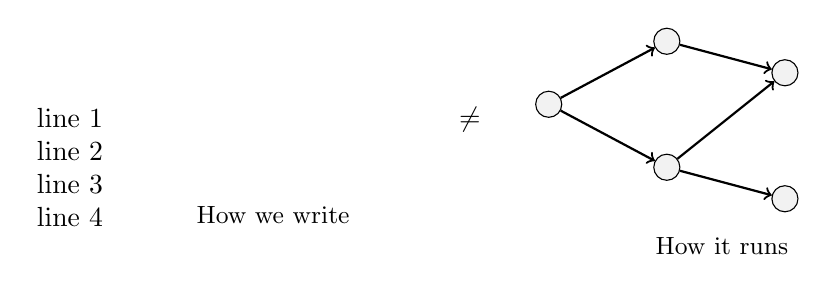
\begin{tikzpicture}[baseline]
    \node[align=left, text width=3cm] (L) {line 1\\line 2\\line 3\\line 4};
    \node[circle, draw, fill=gray!10] (a) at (5,0.8) {};
    \node[circle, draw, fill=gray!10] (b) at (6.5,1.6) {};
    \node[circle, draw, fill=gray!10] (c) at (6.5,0) {};
    \node[circle, draw, fill=gray!10] (d) at (8,1.2) {};
    \node[circle, draw, fill=gray!10] (e) at (8,-0.4) {};
    \draw[->, thick] (a) -- (b);
    \draw[->, thick] (a) -- (c);
    \draw[->, thick] (b) -- (d);
    \draw[->, thick] (c) -- (d);
    \draw[->, thick] (c) -- (e);
    \node at (4,0.6) {$\neq$};
    \node at (1.5,-0.6) {\small How we write};
    \node at (7.2,-1.0) {\small How it runs};
\end{tikzpicture}
\caption{The mismatch between code-as-text and code-as-structure.}
\end{figure}

What code \textit{actually} is, is a set of rules that transform one state into another:
\[
\text{State} \xrightarrow{\text{rules}} \text{State}'
\]

Which is—if we’re honest—a graph rewrite.

Here’s the short list:
\begin{itemize}
    \item Dependencies, data flow, operation ordering—\textbf{graphs}.
    \item State transformations—\textbf{graph rewrites}.
    \item History and conflicts—\textbf{graph merges}.
    \item Parallelism and race conditions—\textbf{graph partitions colliding}.
    \item Debugging and optimization—\textbf{navigating and shortening paths}.
\end{itemize}

The worst graphs are the ones we don't know we're using: undocumented state machines that live only in one engineer's head; the implicit flow Sarah knows but never wrote down; the tribal-knowledge dependency graph that mutates when someone leaves; the mental models that rot while the code keeps moving.

\textbf{Invisible graphs still drive the system—they just do it silently, until they snap.}  
And when they snap, we pay the bill.

I didn't know it yet, but I was staring at the core idea this book is built on:

\textbf{Computation isn't made of instructions. Computation is made of transformations.}

And transformations have shape. And shape is a graph.

\section{From Build Systems to a Theory of Structured Computation}
\label{sec:theory-of-everything}

I spent the next decade chasing the same pattern through every layer of the stack—distributed services, engine rewrites, asset pipelines, migrations. The domain kept changing. The geometry never did. And every problem became clearer once I could draw it.

Once you start thinking in transformations, you stop seeing code as something you ``run'' and start seeing it as something that \textit{moves}. A program is a journey. An execution is a path. A bug is a wrong turn. A merge conflict is two incompatible routes trying to occupy the same space. Concurrency is overlapping travel. Caching is revisiting past locations. Optimization is finding a shorter path. AI reasoning is exploring alternative paths. Simulation is repeated transformation under rules.

Modern software kept growing—multi-threaded, distributed, asynchronous, reactive, stateful, data-heavy, AI-driven—and the old metaphors collapsed under the load. We don’t need new metaphors. We need a new language.

Not a language to replace mathematics or computer science, but one to sit beside them—and let us talk about computation as it actually feels today: structural, dynamic, historical, branching, concurrent, emergent, and made of transformations.

That is what this book is. A language for thinking in transformations. A language for the real shape of software. A language I wish I'd had the day I stared at a broken build system and realized I was seeing the edges of something big.

\section{How State Moves}
\label{sec:how-state-moves}

One of the weirdest things about being a software engineer is how often you find yourself working on a system without knowing what the system \textit{is}.

Not philosophically—literally. You're staring at logs, stack traces, telemetry, exceptions, wire traces, crash dumps, network graphs, build steps, shader compilations, behavior trees—all disconnected snapshots of state—and the entire job boils down to one forbidden question:

\textbf{How did the system get here?}

Nobody documents movement. They document pieces—functions, modules, features, APIs—frozen in time like crime scene photos. But what you actually need is the movie.

And every movie starts the same way: \textbf{Something changes.}

A value updates $\rightarrow$ a message arrives $\rightarrow$ an event fires $\rightarrow$ a collider triggers $\rightarrow$ an asset loads $\rightarrow$ a network packet arrives $\rightarrow$ an AI agent evaluates a condition $\rightarrow$ a file finishes compiling $\rightarrow$ a row mutates $\rightarrow$ a job queues $\rightarrow$ a coroutine yields $\rightarrow$ a thread wakes up.

It's all movement. You're not debugging code—you’re debugging motion.

One day, after chasing a janky asset-pipeline bug that only happened on the third build of the day under full moonlight, I caught myself sketching the system on the whiteboard. And it hit me: I wasn't drawing code. I was drawing state moving through transformations.

It was just boxes and arrows. But it told a story:

\textit{This asset caused that task $\rightarrow$ which triggered that compiler $\rightarrow$ which created that file $\rightarrow$ which fed into that linker $\rightarrow$ which produced that binary $\rightarrow$ which crashed on that device $\rightarrow$ because that metadata was malformed $\rightarrow$ because the dependency graph was wrong $\rightarrow$ because someone "optimized" a build script six months ago.}

None of this was ``business logic.'' None of this was ``gameplay.'' This was just state flowing through a sequence of transformations.

And the more I stared at it, the more obvious it felt: \textbf{Everything in software is just state moving through transformations.}

The behavior wasn’t in the individual pieces. It was in the \textit{connections}.  
Not in the functions, but in the flow.  
Not in the modules, but in the motion.

Every crash, every deadlock, every corrupted asset, every “why is this broken again” moment was just tracing a path until we found where the universe branched wrong.

The only honest representation of software is a map of how state moves.  
Not the class diagram.  
Not the UML.  
Not the architecture deck collecting dust.  
Just:

\[
\text{state} \rightarrow \text{transform} \rightarrow \text{state} \rightarrow \text{transform} \rightarrow \text{state}
\]

—which is, if you zoom out far enough, a graph rewrite.

Suddenly: compilers, build systems, asset pipelines, physics engines, networking, distributed systems, UIs, AI planning, databases, version control, even the goddamn game loop—they all look the same:

\textbf{A world of states, and the rules that transform them.}

This is where \COMPUTER{} really begins. Once you understand movement, you understand computation. And once you can draw movement, you can control it. If you can see the path, you can change it.

\section{Why Structure Emerges Everywhere}
\label{sec:why-structure-emerges}

There’s a moment in every engineer’s life—whether they admit it or not—where they stare at three completely different systems and think: ``Why the hell do these all look the same?''

The domains differ. The problems differ. The technologies differ. And yet—\textit{they rhyme}. They want to be graphs. They want to be structure. They want to be transformations.

That repetition isn’t an accident. It’s a signal.

\subsection{The Physics Engine That Looked Suspiciously Like a Compiler}

Back at that studio—long before I had the vocabulary for any of this—I noticed something odd. Our physics engine's collision pipeline looked… a lot like the compiler pipeline.

\begin{figure}[h]
    \centering
    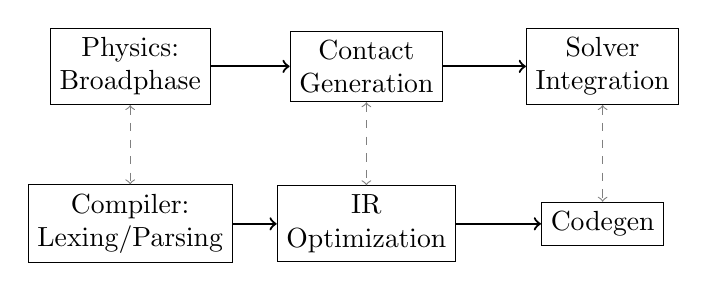
\begin{tikzpicture}[node distance=3cm, auto]
        \node [draw, align=center] (A) {Physics:\\Broadphase};
        \node [draw, align=center, right of=A] (B) {Contact\\Generation};
        \node [draw, align=center, right of=B] (C) {Solver\\Integration};
        
        \node [draw, align=center, below of=A, yshift=1cm] (D) {Compiler:\\Lexing/Parsing};
        \node [draw, align=center, right of=D] (E) {IR\\Optimization};
        \node [draw, align=center, right of=E] (F) {Codegen};
        
        \draw[->, thick] (A) -- (B);
        \draw[->, thick] (B) -- (C);
        \draw[->, thick] (D) -- (E);
        \draw[->, thick] (E) -- (F);
        
        \draw[<->, dashed, gray] (A) -- (D);
        \draw[<->, dashed, gray] (B) -- (E);
        \draw[<->, dashed, gray] (C) -- (F);
    \end{tikzpicture}
    \caption{The structural isomorphism between a physics engine and a compiler pipeline.}
\end{figure}

Totally different domains. Totally different math. Totally different problems. Same shape:  
input $\rightarrow$ transform $\rightarrow$ transform $\rightarrow$ output.  
A pipeline. A DAG. A rewrite sequence.

Later in the book, we’ll see why physics and computation rhyme so well—and why the resemblance might not be a coincidence.

\subsection{The AI Behavior Tree That Looked Like a Build System}

Debugging a behavior tree bug one day—NPC frozen because a leaf node failed silently—I caught myself thinking: ``Why does this feel exactly like tracing build dependencies?''

Pending branches. Cached results. Reactive triggers. Upstream failures. Subtree retries.  
Different skin. Same skeleton.

\subsection{Distributed Systems and Animation Systems}

Years later, working on distributed backend services, the déjà vu hit again: queues, events, fan-out, rollback, replay, scheduling, dependency ordering.  
It felt exactly like the animation system I'd worked on in games.

Different domain. Same geometry.

\subsection{After a While, You Start Asking Different Questions}

First you ask: ``Why does everything look like a graph?''  
Then: ``Is this just how my brain works?''  
Then: ``No seriously—why is this everywhere?''

The answer is simple:

\textbf{Systems that evolve under rules naturally collapse into graph structure.}

If something has parts—and those parts can change—you get a graph.

\begin{itemize}
    \item Atoms bond $\rightarrow$ graph
    \item Functions call each other $\rightarrow$ graph
    \item Assets depend on assets $\rightarrow$ graph
    \item Events trigger events $\rightarrow$ graph
    \item AI nodes activate nodes $\rightarrow$ graph
    \item Game states transition $\rightarrow$ graph
    \item Machines coordinate $\rightarrow$ graph
    \item Humans coordinate $\rightarrow$ graph
\end{itemize}

Structure emerges because dependencies, causality, concurrency, history, and flow \textit{are} structure.  
Rules operating on state create structure.  
So it’s not that your brain is “stuck in graph mode.”  
It’s that engineered systems are \textbf{forced} into graph shape by the nature of change itself.

\section*{The Map vs. The Territory}

Now here’s the grounding point—the thing keeping this book sane.  
Just because engineered systems resemble graphs does not mean the universe literally is one.

\COMPUTER{} doesn’t \textit{start} by redefining physics.  
At this layer of abstraction, it's simply a language for reasoning about engineered systems—software, pipelines, architectures, flows.  

\textit{Whether that same language also describes the universe we live in}  
is a question we’ll revisit in Part VI, once we've built enough machinery to ask it responsibly.

That’s why this chapter exists.  
To show you:

\begin{center}
\textbf{You're not imagining it, and you're not alone.  
The pattern is real—and we're going to formalize it.}
\end{center}

We were trying to force a graph-shaped universe into a linear-shaped hole.

If you can see the geometry of computation, you can redesign the machine itself.

\medskip

\noindent\textbf{Where We Go From Here}

\begin{itemize}
    \item \textbf{Part I} formalizes the substrate—Recursive Metagraphs.
    \item \textbf{Part II} shows how computation moves through it.
    \item \textbf{Part III} gives that movement geometry—distance, curvature, possibility.
    \item \textbf{Part IV} builds machines that exploit this geometry: rewinders, explorers, provers.
    \item \textbf{Part V} connects this all to engineering practice: correctness, concurrency, provenance.
    \item \textbf{Part VI} asks the forbidden question:
    
    \begin{center}
    \textit{If this language explains engineered systems so well…  
    what else might it explain?}
    \end{center}
\end{itemize}

This book is the answer to that question.

\bigskip

\noindent\textbf{Where this leads.}  
The moment you see software as state moving through transformations,  
you need a formal language for describing that motion.

Part I gives us that language.
